\documentclass{article} % For LaTeX2e
\usepackage{nips15submit_e,times}
\usepackage{hyperref}
\usepackage{url}
\usepackage{graphicx}
\usepackage{amsmath}
%\documentstyle[nips14submit_09,times,art10]{article} % For LaTeX 2.09


\title{Predict Closed Questions on Stack Overflow}


\author{
Amritanshu Agrawal, George Mathew\\
Department of Computer Science, NCSU\\
Raleigh, NC 27606 \\
\texttt{\{aagrawa8, george2\}@ncsu.edu} \\
\vspace{-1.0cm}
}

% The \author macro works with any number of authors. There are two commands
% used to separate the names and addresses of multiple authors: \And and \AND.
%
% Using \And between authors leaves it to \LaTeX{} to determine where to break
% the lines. Using \AND forces a linebreak at that point. So, if \LaTeX{}
% puts 3 of 4 authors names on the first line, and the last on the second
% line, try using \AND instead of \And before the third author name.

\newcommand{\fix}{\marginpar{FIX}}
\newcommand{\new}{\marginpar{NEW}}

\nipsfinalcopy % Uncomment for camera-ready version

\begin{document}


\maketitle

% \begin{abstract}
% The abstract paragraph should be indented 1/2~inch (3~picas) on both left and
% right-hand margins. Use 10~point type, with a vertical spacing of 11~points.
% The word \textbf{Abstract} must be centered, bold, and in point size 12. Two
% line spaces precede the abstract. The abstract must be limited to one
% paragraph.
% \end{abstract}

\section{Introduction}

Stack Overflow\footnote{\url{http://stackoverflow.com}} is used by over millions of programmers everyday to obtain answers for their questions. Due to this reason, quality must be safe-guarded to ensure that if new questions are \textit{off topic}, \textit{not constructive}, \textit{not a real question} or \textit{too localized}. These questions should end up being \textbf{closed}. Currently
about $6\%$ of all new questions end up being "closed". In this project, we predict if a question will be closed based on the attributes and the reason why it will be closed. The possible reasons we plan on analyzing are
\begin{itemize}
    \item \textbf{Open - 50\%} : Question is not marked closed.
    \item \textbf{Off Topic (OT) - 17\%} : If the question is not related to the topics allowed in a certain StackExchange website.
    \item \textbf{Not Constructive (NC) - 18\%} : If the question is open ended and can have many equally valid answers.
    \item \textbf{Not a Real Question (NRQ) - 10\%}: If the question has responses asking for clarification or additional information, or responses that are at best partial answers.
    \item \textbf{Too Localized (TL) - 5\%}: If the question cannot possibly be answered because nobody participating in the site is likely to know the answer.
\end{itemize}


\subsection{Dataset}
The data used for this project is available from kaggle\footnote{\url{https://goo.gl/aVrXiE}}. It includes train data which contains 3,664,927 posts and train sample data consisting of 178,351 posts. Full train data
and sample train data distribution~\cite{lezina2013predict} on closed reasons is shown in table 1. Each post contains the creation time, user-id of the created user, title of the question, body of the question in markdown, tags for the question and the status of the question. The training data is in a .csv file of 3.5 GB consisting of the attributes described above. The test data is also in a .csv file of 800 KB. We have multi-class classification problem. We are saying open as one class and close if they are NRQ, NC, OT, TL. We are seeing highly imbalanced classes.

\begin{table}[!htbp]
\begin{center}
\begin{tabular}{|c|c|c|c|c|c|}        
        \hline
        Dataset & NRQ & NC & OT & Open & TL \\ [0.5ex]
        \hline
        Train & 38622 & 20897 & 20865 & 3575678 & 8910 \\ [0.5ex]
        \hline
        Sample & 38622 & 20897 & 20865 & 89337 & 8910 \\ [0.5ex]
        \hline
\end{tabular}
\end{center}
\caption{Training data distribution over categories}
\label{tb:dataset}
\vspace{-2mm}
\end{table}

\section{Background}
Questions on StackOverflow are closed by user voting. So user's feedback is very important component also it's a valuable source of post quality. In~\cite{agichtein2008finding} user relationships were analyzed to gain significant amount of quality information.  The main idea was that ``good" users write ``good" answers. This idea can be propagated onto the questions that peoples who do not asks "bad" questions are less unlikely to do so in the future. Their features for text quality analysis were helpful because one of the close reason - not constructive - is essentially a conversational question.

In~\cite{harper2009facts} authors classified questions as conversational and informational. In their work they divided peoples into two categories: answer people, who answers many questions and discussion peoples who interact often with other discussion people. Authors~\cite{mendes2009socializing} showed that almost the same user interaction features are significant during classification of a question as social and non-social.

\section{Method}
\subsection{Preprocessing}
\label{preprocess}

Our data contains mostly text and we employed different preprocessing steps to get rid of unusual words. Our steps include:
\begin{itemize}
    \item \textbf{Tokenization:} Tokenization occurs at the word level. For this good regular expressions are used. %\begin{displaymath}
    %<(.*?)>|\backslash %n|(\\(.*?){)|}|[\#!\$\%\wedge\&*()\_+|~\^%\-<>/={}\[\],:\";<>?,.\/\\]|[@]
    %\end{displaymath}
    Punctuation and whitespace are not included in the resulting list of tokens. Even removal of numbers as they don't mean anything.
    \item \textbf{Email and urls removal:} The email ids and urls of different types are removed.
    \item \textbf{Stopword removal:} Stop words removal using NLTK toolkit\footnote{http://www.nltk.org/book/ch02.html}~\cite{bird2009accessing} : ignore very common short words such as  ``and'' or ``the''.
    \item \textbf{Stemming:} Porter's stemming filter~\cite{porter1980algorithm}: delete uninformative word endings; e.g. after stemming, all the following words would be rewritten
  to ``connect'': ``connection'', ``connections'',
``connective'',          
``connected'',
  ``connecting''.
\end{itemize}

\subsection{Featurization}
\label{features}

Once preprocessing is done, we converted textual blob to a feature matrix. There are various standard state of art methods which have been useful in text mining. Some of those mentioned are:-

\begin{itemize}
  \item \textbf{Bag-of-words:} In this model, a text (such as a sentence or a document) is represented as the bag (multiset) of its words. The (frequency of) occurrence of each word is used as a feature for training a classifier.
    \item \textbf{Tf-idf feature selection:} Tf–idf, short for term frequency–inverse document frequency, is a numerical statistic that is intended to reflect how important a word is to a document in a collection or corpus. If a word occours $w$ times
  and is found in $d$ documents  and there
  are $W,D$ total number of words and documents respectively, then tf-idf is scored
  as follows:
  \[
  \mathit{tfidf}(w,d)=   \frac{w}{W} *\log{\frac{D}{d}}\]
  \item \textbf{L2 Row normalization:} The Euclidean norm (L2 normalization) assigns to each vector the length of its arrow. Since, we know each document can have different length in a model because of different set of words. L2 row normalization is done to make each row of same length as a feature matrix. And the added advantage is to reduce the vocabulary size dramatically.
  \item \textbf{LDA:} Latent Dirichlet Allocation~\cite{blei2003latent} is a widely-used topic modeling algorithm.  LDA reduces any document to a fixed set of real-valued features—the posterior Dirichlet parameters associated with the document (which we call as document-topic distribution).
\end{itemize}

\subsection{Classifiers}
\label{classifier}

There are various standard classifiers which are used for text mining classification. They are:
\begin{itemize}
    \item \textbf{SVM:} A Support Vector Machine (SVM) is a discriminative classifier formally defined by a separating hyperplane. In other words, given labeled training data (supervised learning), the algorithm outputs an optimal hyperplane which categorizes new examples. It comes with different kernels like linear, radial bayes function to transform data into multidimensions and finding the right hyperplane for good distinction.
    \item \textbf{Logisitc Regression:} The logistic regression is a predictive analysis. Logistic regression is used to describe data and to explain the relationship between one dependent binary variable and one or more metric (interval or ratio scale) independent variables.
    \item \textbf{Naive Bayes:} Naive Bayes classifiers are a family of simple probabilistic classifiers based on applying Bayes theorem with strong (naive) independence assumptions between the features.
    \item \textbf{Decision trees:} Decision Tree Classifier poses a series of carefully crafted questions about the attributes of the test record. Each time  it receive an answer, a follow-up question is asked until a conclusion about the class label of the record is reached. In our experiment we use CART\cite{olshen1984classification} which is one of the modern decision tree which is similar to  the ID3 decision tree algorithm.
\end{itemize}

\subsection{Evaluation Measures}
\label{evaluation}

Since, this is a multi-class classification problem, we represent the predictions using a confusion matrix where a `positive' output is the class under study and a `negative' output is all the other classes. The confusion matrix is shown in figure \ref{fig:cmatrix}.

\begin{figure}[!htpb]
    \centering
    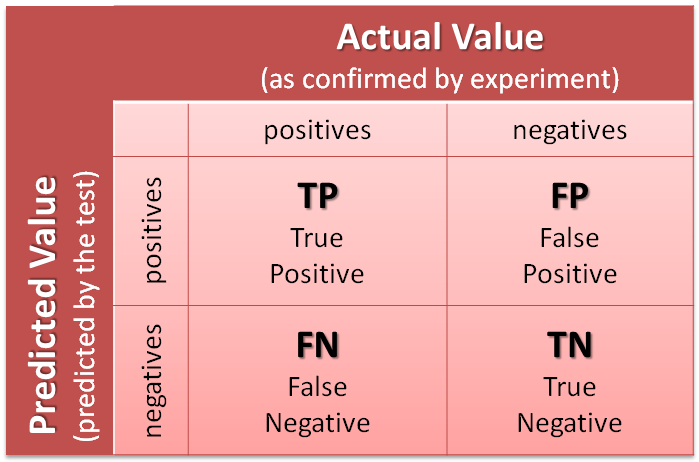
\includegraphics[scale=0.25]{figs/cmatrix}
    \caption{Confusion Matrix}
    \label{fig:cmatrix}
\end{figure}

We use the following evaluation measures.
\begin{itemize}
    \item \textbf{Precision}: Ratio of True Positives in all values positively predicted.
    \[Precision(prec) = \dfrac{TP}{TP + FP}\]
    \item \textbf{Recall}: Ratio of True Positives in all values actually positive.
    \[Recall(rec) = \dfrac{TP}{TP + FN}\]
    \item \textbf{F1 score}: Harmonic mean of precision and recall.
    \[F1 = \dfrac{2*prec*rec}{prec + rec}\]
    \item \textbf{Accuracy}: Ratio of true predictions to total number of predictions.\\
    \[Accuracy = \dfrac{TP + TN}{TP + FP + FN + TN}\]
\end{itemize}


\section{Experiment}
We implemented our methods using python and libraries built on python like scikit-learn\footnote{\url{http://scikit-learn.org/}} and NLTK to develop the project. We performed all the preprocessing steps mentioned in section~\ref{preprocess}. For featurization, we selected 3 different set of experiments based on our intuition of reducing the large vocabulary size. They are: 1) Bag of Words with L2 row norm pruned to 4000 features. 2) TF-IDF with L2 row norm pruned to 4000 features. 3) LDA with number of topics $= 500$. We compared our results with all the mentioned classifiers in section~\ref{classifier}. We ran this experiment with stratified 5-fold cross validation. We used stratified since, this dataset contains highly unbalanced classes. The majority class being open () For comparison we are reporting results with respect to precision, recall, f1 score and accuracy. Since the problem, is multi-class classification we set the predicting class as positive and all the other classes as negative. The resulting confusion matrix is generated using this definition of positive and negative.

For all our methods we preset the parameters required for each of them by iterating over a set of parameters and selecting the best parameter whilst applying our engineering judgement. :

\begin{itemize}
    \item \textbf{Logistic Regression}: thresholding function =  sigmoid
    \item \textbf{Naive Bayes}: Smoothing Parameter($\alpha$) = 1.0
    \item \textbf{Linear SVM}: Default Parameters
    \item \textbf{RBF SVM}: Kernel Coefficient($\gamma$) = 0.8
    \item \textbf{CART}: Criterion = gini,  min\_samples\_split=2, min\_samples\_leaf=1 
\end{itemize}

All the experiments have a random seed of 1 to ensure repeatability. The code is deployed on NCSU - High Performance Computing which is an Intel Xeon based Linux cluster with parallel computing on 16 cores. The source code, data and all the results are available online\footnote{\url{https://github.com/amritbhanu/OpenClosedSO_P34/}} and highly recommend users to reproduce our results to ensure its reproducibility and repeatability.

\section{Results}

\subsection{Bag of Words + L2-norm pruned to 4000 features}
\begin{table}[!htpb]
    \centering
    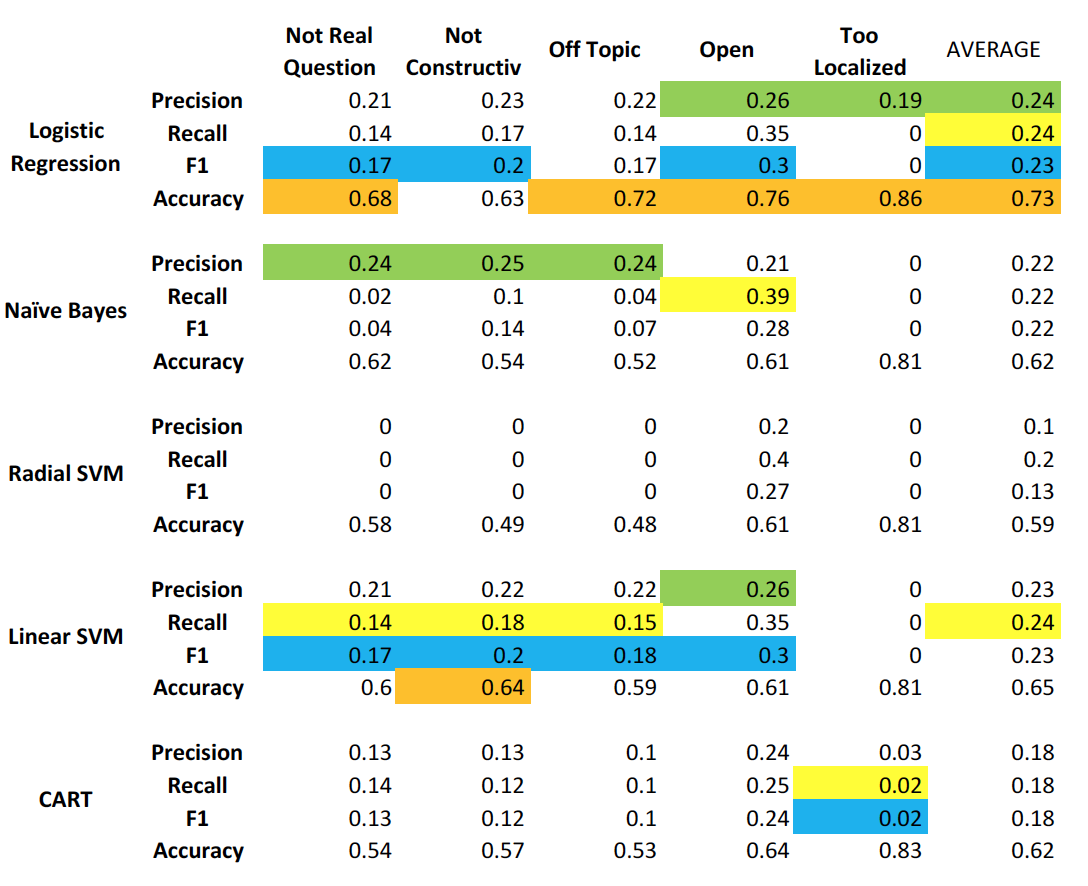
\includegraphics[scale=0.6]{figs/BOW}
    \caption{Bag of Words + L2-norm pruned to 4000 features}
    \label{tab:bow}
\end{table}

For our first set of experiments, we use the Bag Of Words model as our primary featurizer. This converts the pre-processed document into a vector of frequencies. Post this, we normalize the vector using L2 normalization and then select the top 4000 features. Table \ref{tab:bow} shows the evaluation results of the 5 classifiers under study using the this featurization pipeline.


\subsection{TF-IDF + L2-norm pruned to 4000 features}
\begin{table}[!htpb]
    \centering
    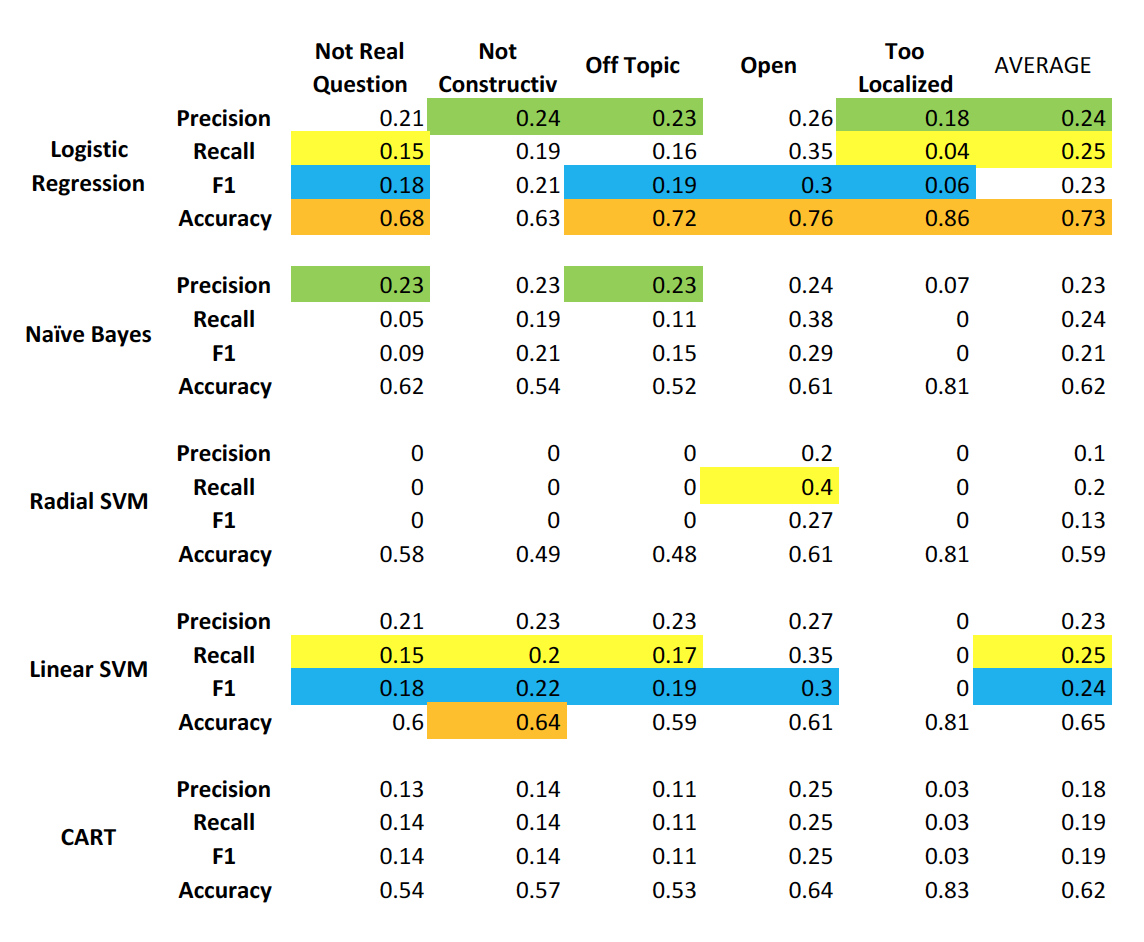
\includegraphics[scale=0.6]{figs/TFIDF}
    \caption{TF-IDF + L2-norm prunted to 4000 features}
    \label{tab:tfidf}
\end{table}
We then replace the Bag of Words featurizer with the TF-IDF featurizer. Here the tokens are ranked based on their term frequency and inverse document frequency in the corpus. we normalize the vector using L2 normalization and then select the top 4000 features. Table \ref{tab:tfidf} shows the evaluation results of the 5 classifiers under study using the this featurization pipeline.


\subsection{LDA - k=500}
\begin{table}[!htpb]
    \centering
    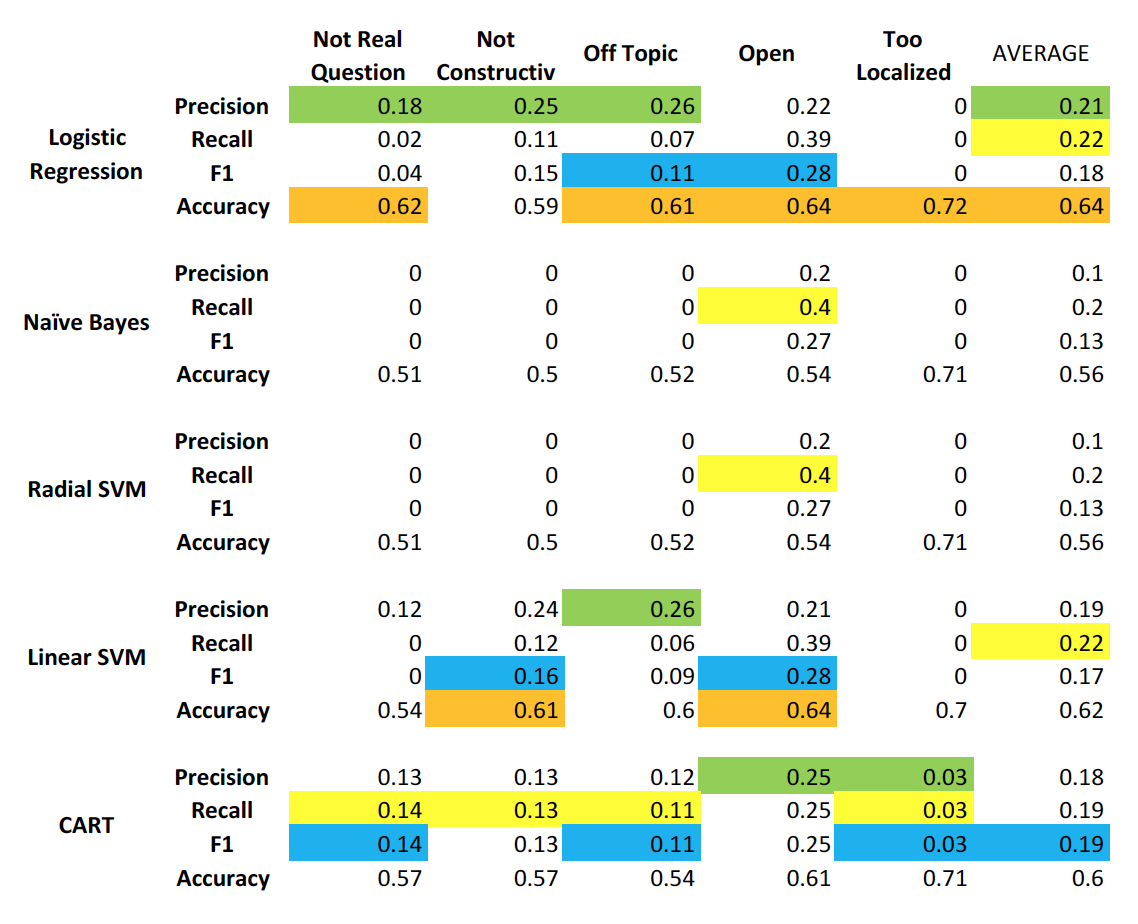
\includegraphics[scale=0.6]{figs/LDA}
    \caption{LDA with 500 topics}
    \label{tab:lda}
\end{table}
Here we use LDA to model the corpus using 500 topics and we represent each document with its topic distribution and we then classify the documents. Table \ref{tab:lda} shows the results of the 5 classifiers where LDA was used as a featurizer.


\subsection{Observations \& Inference}

The results for the experiments are presented in Table \ref{tab:bow}, Table \ref{tab:tfidf} \& Table \ref{tab:lda}. Each table presents the  value of Precision, Recall, F1 score and Accuracy over a 5 fold stratified cross validation rig. Columns 3-7 in each table shows the measures for each of the 5 classes in the dataset and the last column shows the weighted average of the measure where each row has a weight equal to the proportion of classes in the training data.

From the tables, we can draw the following observations and inference

\begin{itemize}
    \item We see very low numbers of precision, recall and fscore. That is due to large sample size (3 million samples) and dramatic feature reduction.
    \item The runtimes were in days (approx 2 days) on HPC for running 5 learners and each learner with stratified 5 fold cross evaluation.
    \item Logistic Regression has relatively one of the better values for all three measures compared to other methods. This is because the data might best split using a linear hyper plane
    \item Naive Bayes has a high recall for two of the closed classes(Not constructive \& Off Topic) and low recall for other closed classes. Generative classifiers like Naive Bayes classifiers are capable of handling closed classes with large samples but fail for closed classes with less samples.
    \item SVM with RBF kernel has the lowest precision for all the classes and every featurization technique. This might be because this dataset cannot be modeled using a radial kernel.
    \item SVM with Linear kernel has the best average precision and relatively high value of recall. Similar to logistic regression, the dataset might be best split using a linear hyper plane.
    \item Decision Tree using with RBF kernel has the lowest recall for all the classes and the lowest average recall. Rule based classifiers perform poorly due to the large diversity within the data and large number of features.
    \item All the methods perform poorly on classifying the ``Too localized'' class as seen by its low precision, recall and F1 values. This is due to the less number of samples for the ``Too localized'' class as compared to other classes(less than 5\%).
\end{itemize}

\section{Conclusion \& Future Work}

In this study, we try to classify stack-overflow questions as open and closed(reasons for closed) questions. We use 4 predictive classifiers (Decision Tree, Logistic Regression, Linear \& Radial SVM) and 1 generative classifier(Naive Bayes) to predict the questions. We observe that choosing a generative or predictive classifier does not make a difference in prediction. Radial SVM has the lowest precision as the data might not be transformed aptly as a  radial function. CART produces the worst recall, which can also highlight that the data cannot be represented as rules(since Decision Trees are Rule Based Classifiers). Linear models produces the best results as seen by Logistic Regression and Linear SVM. This might be because the data can be best split in a linear manner and linear separation is known to have the lowest overfit.

Overall, we see that the overall performance is very low and largely independent of the model chosen. Thus, better results should be obtained by incorporating better feature extraction techniques. Although we use standard text mining pre-processing techniques, we will now include L2-Normalization pruned to larger feature set, TF-IDF Vectorizer over the Bag Of Words Vectorizer and n-gram model to improve the classification accuracy. We know LDA algorithm is quite unstable and depends on its number of topic size. We should be tuning this parameter to find the best fit. And since our classes are highly imbalanced we will try doing SMOTE ~\cite{chawla2002smote} which is a synthetic minority over sampling technique.

The winners of this kaggle competition used a 10-gram model for prediction. Using such markov chain based classifiers will yield better results.


\bibliographystyle{abbrv}
\medskip
\bibliography{ref}

\end{document}